\documentclass{beamer}

\usecolortheme[named=blue]{structure}

\mode<presentation>
{
  \usetheme{Warsaw}
  \setbeamercovered{transparent}
  \setbeamertemplate{items}[ball]
  \setbeamertemplate{theorems}[numbered]
  \setbeamertemplate{footline}[frame number]
}

\usepackage{beamerthemesplit}
\usepackage{hyperref}
\XeTeXlinebreaklocale "zh"
\XeTeXlinebreakskip = 0pt plus 1pt
\usepackage[cm-default]{fontspec}
\usepackage{xunicode,xltxtra}
\usepackage{indentfirst}
\usepackage{xeCJK}
\usepackage{graphicx}
\usepackage{algorithm}
\usepackage{algpseudocode}
\usepackage{amsmath}
\usepackage{xcolor}
\usepackage{listings}
\usepackage{fancyvrb}
\usepackage{tabularx}

\setsansfont{Kai} 

\XeTeXlinebreaklocale "zh"
\XeTeXlinebreakskip=0pt plus 1pt minus 0.1pt


\title
{多核可扩展操作系统内核的实现与研究}
\subtitle{开题报告}
  \author{计92 陈宇恒\\指导老师:陈渝}
\institute{清华大学计算机系}

\begin{document}
%-----------------------------------------------------------------------------80
  \frame
  {
    \titlepage
  }

\section*{大纲}
\frame{\tableofcontents }

\section{课题背景}
	\frame{
		\frametitle{已有操作系统的问题}
	  当前基于AMD64/X86\_64架构的多核系统已经得到广泛应用。但随着40核甚至
	  80核的NUMA系统的出现,对已有操作系统的多核可扩展性提出了苛刻的要求。

		\begin{itemize}
			\item
		由于已有操作系统多数是由单核系统演化而来,在设计之初就使用了一些
		不具有多核扩展性的数据结构来维护VMA、DCACHE、MountTable等内核关键
		数据结构。这导致Linux等操作系统在20核以上硬件系统上表现不佳,甚至
		出现性能下降;
			\item 一些同步原语没有为重核架构优化,例如Linux的Spinlock
				实现在重核架构上导致代价高昂的Cache同步协议开销;
			\item
				操作系统设计上的问题。例如Linux中各个Core共享页表,
				在一些应用下造成不必要的TLB shootdown。
		\end{itemize}
		鉴于这些问题,我们希望重新设计一个小型实验性操作系统,从根本上解决这些
		问题。

	}
	\frame{
		\frametitle{Linux中VMA多核扩展性}
		如Linux中的VMA结构对map和unmap操作就不具有多核可扩展性\footnote[frame]{\scriptsize{Austin T. Clements, M. Frans Kaashoek, and Nickolai Zeldovich.
			\\RadixVM: Scalable address spaces for multithreaded
		applications.}}:
		\begin{figure}[ht]
			\begin{center}
				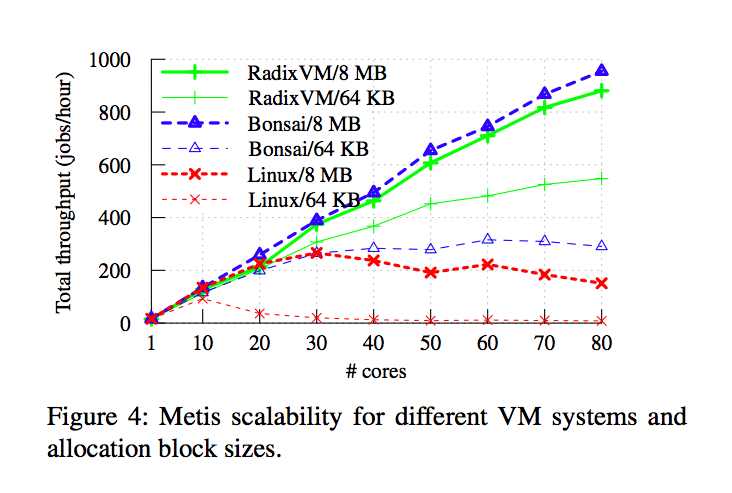
\includegraphics[width=0.7\textwidth]{linux.png}
			\end{center}
			\label{fig:vma}
		\end{figure}
	}

	\frame{
		\frametitle{毕设工作的基础}
		多核系统的优化是现在热门的研究课题之一,本毕设工作可以基于以下成果:
		\begin{itemize}
			\item MIT PDOS xv6/SCK实验操作系统
			\item 崔岩学长:面向多核架构的操作系统可扩展性研究
			\item
				王乃峥学长:基于消息传递的系统服务优化
				(FlexSC syscall实现)
		\end{itemize}
	}

\section{毕设工作重点}

	\frame{
		\frametitle{总体目标}
	  本课题希望实现具有以下特性的小型操作系统:
	  \begin{itemize}
		  \item
			  在qemu(多核模拟),kvm(多核)和真机(多核)上正常运行
		\item 识别多核NUMA架构
		\item
			完善的性能数据采集功能,包括Qemu上和真机上的性能数据采集
		\item 易于实现Per-Core Pagetable、FlexSC等实验性多核技术
	  \end{itemize}
  	}

	\frame{
		\frametitle{工作计划}
		重头实现一个操作系统是比较有挑战性的,但我们已有uCore、MIT的xv6/SCK等
		实验OS做参考。

		毕设工作的总体计划为先在我们的实验OS中实现MIT xv6多核系统中
		的基本功能,然后实现优化的Syscall,Message Passing等新机制。
		
		具体计划如下:
		\begin{itemize}
			\item 进一步理解AMD64/X86\_64系统架构 (Week 1-4)
			\item
				完成NUMA架构的CPU,内存支持,以及完成APIC,IOAPIC等
				体系结构特定代码 (Week 5-6)
			\item 完成可以在多核上工作的内存管理、调度器等模块
				(Week 7-9)
			\item 在我们的OS上实现MIT PDOS实验室的最新 
				研究成果,设计基于每个core的物理内存,虚拟内存,调度管理
				,RCU同步互斥机制等各个模块(Week 10-14)
		\end{itemize}
	  	本毕业设计也与MIT PDOS实验室的最新工作紧密联系。

	}

	\frame{
		\frametitle{前四周工作}
		前四周以调研和对AMD64多核系统了解为主,完成了以下代码工作:
		\begin{itemize}
			\item ACPICA库移植
			\item LAPIC初始化
			\item CPU和NUMA节点信息读取
		\end{itemize}

	}

\section{相关工作}
	\frame{
		\frametitle{MIT PDOS实验室 -- 2013}
		\begin{block}
		\bf{RadixVM: Scalable address spaces for multithreaded
		applications} \\
		Austin T. Clements, M. Frans Kaashoek, and Nickolai
		Zeldovich
		\end{block}
		基于xv6实验OS设计了一个全新的虚拟存储管理模块RadixVM,在80核机器上获得
		了几乎线性的加速比。主要工作:
		\begin{itemize}
			\item 使用Refcache替代传统的atomic inc/dec操作
			\item 使用改进Radix Tree实现VMA映射,主要
				难点在空间压缩上
			\item 跟踪每个Core的VMA使用,只对必要的Core进行
				TLB Shootdown
		\end{itemize}
	}

	\frame{
		\frametitle{MIT PDOS实验室 -- OSDI2010}
		\begin{block}
		\bf{An Analysis of Linux Scalability to Many Cores}\\
		MIT CSAIL
		\end{block}
		针对Exim, memcached, Apache, PostgreSQL, gmake,
		Psearchy和MapReduce这几个常见应用,分析了他们在48核Linux上的性能表现,
		总结了10多个造成多核性能瓶颈的关键代码点,并对Linux做出对于修改。
		他们修改了Linux2.6.35-rc5,在多核性能表现上有显著提升。
	}

	\frame{
		\frametitle{其他资料}
		\begin{block}
		\bf{基于消息传递的系统服务优化}\\
		王乃峥
		\end{block}
		把Message-Passing的思想应用到传统操作系统之中,通过
		修改Linux内核和Glibc,实现了用户态多线程,在此基础上实现了一种新
		的调度和Syscall方式。
	}


\end{document}

